%iffalse
\let\negmedspace\undefined
\let\negthickspace\undefined
\documentclass[journal,12pt,onecolumn]{IEEEtran}
\usepackage{cite}
\usepackage{amsmath,amssymb,amsfonts,amsthm}
\usepackage{algorithmic}
\usepackage{graphicx}
\usepackage{textcomp}
\usepackage{xcolor}
\usepackage{txfonts}
\usepackage{listings}
\usepackage{enumitem}
\usepackage{mathtools}
\usepackage{gensymb}
\usepackage{comment}
\usepackage[breaklinks=true]{hyperref}
\usepackage{tkz-euclide} 
\usepackage{listings}

\usepackage{booktabs}
\usepackage{pgfplots}
\usepackage{gvv}                                        
\usepackage[latin1]{inputenc}     
\usepackage{xparse}
\usepackage{color}                                            
\usepackage{array}                                            
\usepackage{longtable}                                       
\usepackage{calc}                                             
\usepackage{multirow}
\usepackage{multicol}
\usepackage{hhline}                                           
\usepackage{ifthen}                                           
\usepackage{lscape}
\usepackage{tabularx}
\usepackage{array}
\usetikzlibrary{patterns}
\usepackage{siunitx}
\pagestyle{empty}
\usetikzlibrary{calc}
\usepackage[margin=1in]{geometry}
\usepackage{pgffor}
\usepackage{float}
\usepackage{pgf-pie}
\newtheorem{theorem}{Theorem}[section]
\newtheorem{problem}{Problem}
\newtheorem{proposition}{Proposition}[section]
\newtheorem{lemma}{Lemma}[section]
\newtheorem{corollary}[theorem]{Corollary}
\newtheorem{example}{Example}[section]
\newtheorem{definition}[problem]{Definition}
\newcommand{\BEQA}{\begin{eqnarray}}
\newcommand{\EEQA}{\end{eqnarray}}
\newcommand{\define}{\stackrel{\triangle}{=}}
\theoremstyle{remark}
\newtheorem{rem}{Remark}
% Marks the beginning of the document
\pgfplotsset{compat=1.18}
\begin{document}

\bibliographystyle{IEEEtran}
\vspace{3cm}


\title{2020-CE-'53-65'}
\author{EE24BTECH11023}
%\maketitle
%\newpage
%\bigskip
\maketitle

{\let\newpage\relax\maketitle}

\renewcommand{\thefigure}{\theenumi}
\renewcommand{\thetable}{\theenumi}
\setlength{\intextsep}{10pt} % Space between text and floats


\numberwithin{equation}{enumi}
\numberwithin{figure}{enumi}
\renewcommand{\thetable}{\theenumi}

\begin{enumerate}
    \item A gaseous chemical has a concentration of 41.6 $\mu$mol/m$^3$ in air at 1 atm pressure and temperature 293 K. The universal gas constant is $82.05 \times 10^{-3} \, \text{m}^3 \cdot \text{atm} / (\text{mol} \cdot \text{K})$. Assuming the ideal gas law is valid, the concentration of the gaseous chemical (in ppm ,round off to one decimal place) is {\underline{\hspace{2cm}}}.

    \item A stream with a flow rate of $5m ^ 3$ / s is having an ultimate BOD of 30 mg/litre. A wastewater discharge of $0.2m ^ 3 / s$ having BODs of 500 mg/litre joins the stream at a location and instantaneously gets mixed up completely. The cross-sectional area of the stream is $40m ^ 2$ which remains constant. BOD exertion rate constant is 0.3 per day (logarithm base to e). The BOD (in mg/litre, round off to two decimal places) remaining at 3 km downstream from the mixing location, is
    \item The lengths and bearings of a traverse PQRS are given as follows:
   \begin{table}[H]
        \centering
        \begin{center}
    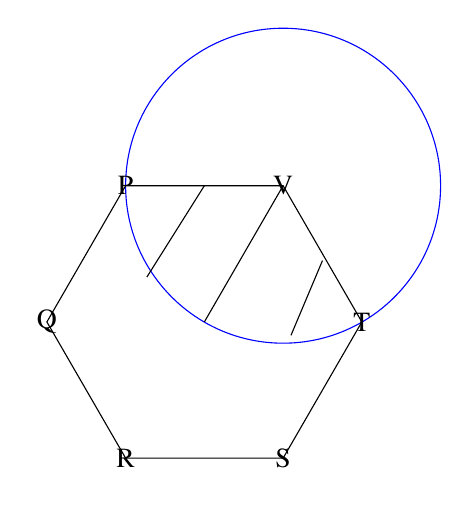
\begin{tikzpicture}
            \draw[blue] (2,3.46) circle (2);
            \draw(1,3.46)--(0.27,2.3);
            \draw(2,3.46)--(1,1.73);
            \draw(2.5,2.509)--(2.1,1.56);
        \draw (0,0) -- (2,0) -- (3,1.73) -- (2,3.46) -- (0,3.46) -- (-1,1.73) -- cycle;
        \node at (0,0) {R};
        \node at (2,0) {S};
        \node at (3,1.73) {T};
        \node at (2,3.46) {V};
        \node at (0,3.46) {P};
        \node at (-1,1.73) {Q};
    \end{tikzpicture}
    \end{center}  
    \end{table}
    The length of line segment SP (in m, round off to two decimal places),is {\underline{\hspace{2cm}}}.
    \item Rescue teams deployed {\underline{\hspace{2cm}}} disaster-hit areas combat {\underline{\hspace{2cm}}} a lot of difficulties to save the people. 
    \begin{enumerate}
        \item with, at
        \item in, with
        \item with, with
        \item to, to
    \end{enumerate}
    \item Select the most appropriate word that can replace the underlined word without changing the meaning of the sentence:\\Nowadays, most children have a tendency to \underline{belittle} the legitimate concerns of their parents.
    \begin{enumerate}
        \item disparage
        \item applaud
        \item reduce
        \item begrudge
    \end{enumerate}
    \item Select the word that fits the analogy:\\
    Partial : Impartial :: Popular :
    \begin{enumerate}
        \item Impopular
        \item Dispopular
        \item Mispopular
        \item Unpopular
    \end{enumerate}
    \item After the inauguration of the new building, the Head of the Department (HoD) collated faculty preferences for office space.P wanted a room adjacent to the lab.Q wanted to be close to the lift. R wanted a view of the playground.S wanted a corner office.
    \begin{enumerate}
        \item \begin{figure}[H]
        \centering
        \input{figs/Q7A.tex}  
    \end{figure}
        \item \begin{figure}[H]
        \centering
        \input{figs/Q7B.tex}
    \end{figure}
    \item \begin{figure}[H]
        \centering
         \begin{tikzpicture}
            \draw (0.3,0) -- (4,0) -- (4,2) -- (3.5,2) --(3.5,1.3)--(3.2,1.3)--(3.2,2) --(2.9,2)--(2.9,3)--(2.7,3)--(2.7,1.3)--(2.4,1.3)--(2.4,2.5)--(2,2.5)--(2,1.6)--(1.6,1.6)--(1.6,1.8)--(1.8,1.8)--(1.8,3.4)--(1.4,3.4)--(1.4,2)--(0.9,2)--(0.9,2.6)--(0.6,2.6)--(0.6,2)--(0.3,2)--(0.3,0) -- cycle;
        \end{tikzpicture}
 
    \end{figure}
    \item \begin{figure}[H]
        \centering
         \begin{tikzpicture}
            \draw (0.3,0) -- (4,0) -- (4,2) -- (3.7,2) --(3.7,2.5)--(3.5,2.5)--(3.5,2) --(3,2)--(3,3)--(2.6,3)--(2.6,1.7)--(2,1.7)--(2,1.9)--(2.2,1.9)--(2.2,2.5)--(1.8,2.5)--(1.8,1.4)--(1.4,1.4)--(1.4,2.6)--(1.2,2.6)--(1.2,2)--(1,2)--(1,1.4)--(0.8,1.4)--(0.8,2)--(0.3,2)--(0.3,0) -- cycle;
        \end{tikzpicture}

    \end{figure}
    \end{enumerate}
    \item If $f(x) = x^2$ for each $x \in (-\infty, \infty)$, then $\frac{f(f(f(x))}{f(x)}$ is equal to:
    \begin{enumerate}
        \item $f(x)$
        \item $(f(x))^2$
        \item $(f(x))^3$
        \item $(f(x))^4$
    \end{enumerate}
\section*{Q6-Q10 carry two marks each.}
    \item Nominal interest rate is defined as the amount paid by the borrower to the lender for using the borrowed amount over a specific period of time. Real interest rate calculated on the basis  of actual value(inflation-adjusted), is approximately equal to the difference between the nominal rate and the expected rate of inflation in the economy.\\ Which of the following assertions is best supported by the cbove information?
    \begin{enumerate}
        \item Under high inflation, real interest rate is low and borrowers get benefited.
        \item Under low inflation, real interest rate is high and borrowers get benefited.
        \item Under high inflation, real interest rate is low and lenders get benefited.
        \item Under low inflation, real interest rate is low and borrowers get benefited.
    \end{enumerate}
    \item For the year 2019, which of the previous year's calendar can be reused?
    \begin{enumerate}
        \item 2011
        \item 2012
        \item 2013
        \item 2014
    \end{enumerate}
    \item The ratio of 'the sum of odd positive integers from 1 to 100' to 'the sum of even positive integers from 150 to 200' is {\underline{\hspace{2cm}}}.
    \begin{enumerate}
        \item 45:95
        \item 1:2
        \item 50:91
        \item 1:1
    \end{enumerate}
    \item In a school of 1000 students, 300 students play chess, 600 students play football.If 50 students play both chess and football, the number of students who play neither is {\underline{\hspace{2cm}}}.
    \begin{enumerate}
        \item 200
        \item 150
        \item 100
        \item 50
    \end{enumerate}
    \item The monthly distribution of 9 Watt LED bulbs sold by two firms X and Y from January to June 2018 is shown in the pie-chart and corresponding table. If the total number of LED bulbs sold during April-June 2018 is 50,000, then the number of LED bulbs sold by the firm Y during April-June 2018 is {\underline{\hspace{2cm}}}
     \begin{table}[H]
        \centering
        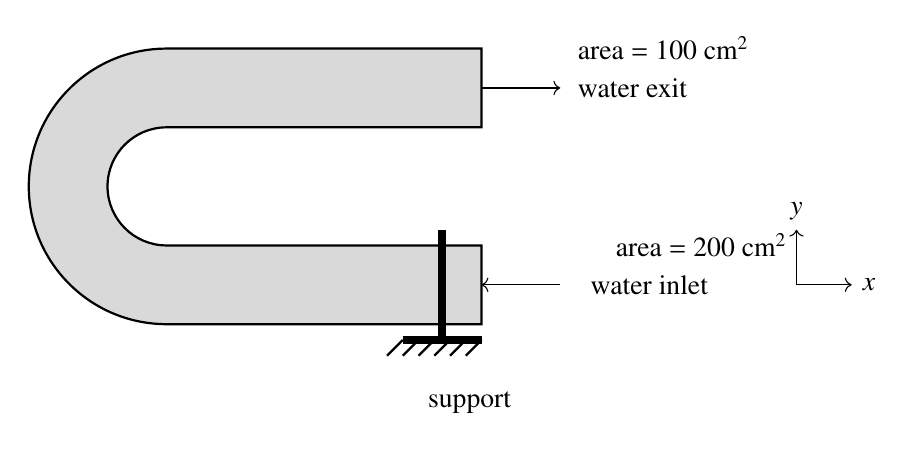
\begin{tikzpicture}
    \draw[thick, fill=gray!30] (0,0.5) -- (4,0.5) -- (4,1.5) -- (0,1.5) arc[start angle=270, end angle=90, radius=0.75] -- (0,3) -- (4,3) -- (4,4) -- (0,4) arc[start angle=90, end angle=270, radius=1.75]--(0,0.5) -- cycle;
    \draw[<-] (4,1) -- (5,1);
    \draw[->] (4,3.5) -- (5,3.5); 
    \node at (4.5,-0.5) [left] {support};
    \draw[line width=1mm](3.5,0.3)--(3.5,1.7);
    \draw[line width=1mm](3,0.3)--(4,0.3);
    \draw[thick](3,0.3)--(2.8,0.1);
    \draw[thick](3.2,0.3)--(3,0.1);
    \draw[thick](3.4,0.3)--(3.2,0.1);
    \draw[thick](3.6,0.3)--(3.4,0.1);
    \draw[thick](3.8,0.3)--(3.6,0.1);
    \draw[thick](4,0.3)--(3.8,0.1);
    \node at (7,1) [left] {water inlet};
    \node at (8,1.5) [left] {area = 200 cm$^2$};
    \node at (5.1,3.5) [right] {water exit};
    \node at (5.1,4) [right] {area = 100 cm$^2$};
    \draw[->] (8,1) -- ++(0.7,0) node[right] {$x$};
    \draw[->] (8,1) -- ++(0,0.7) node[above] {$y$};
\end{tikzpicture}

  
    \end{table}
\begin{figure}[H]
        \centering
        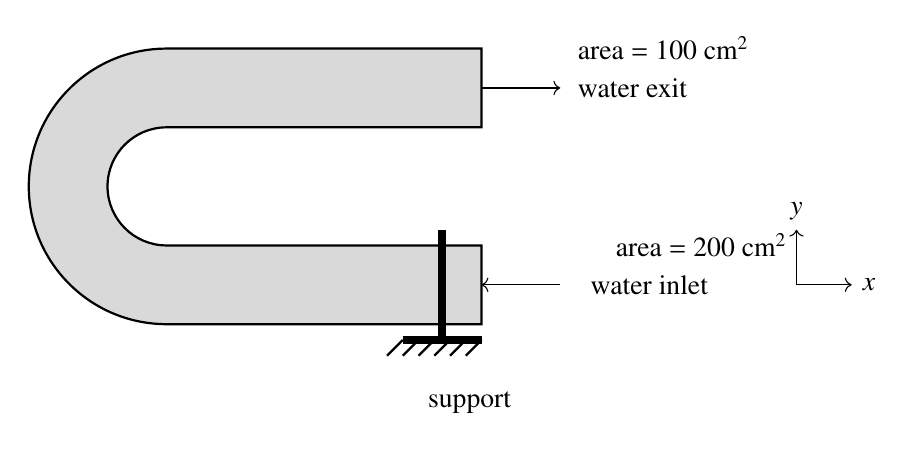
\begin{tikzpicture}
    \draw[thick, fill=gray!30] (0,0.5) -- (4,0.5) -- (4,1.5) -- (0,1.5) arc[start angle=270, end angle=90, radius=0.75] -- (0,3) -- (4,3) -- (4,4) -- (0,4) arc[start angle=90, end angle=270, radius=1.75]--(0,0.5) -- cycle;
    \draw[<-] (4,1) -- (5,1);
    \draw[->] (4,3.5) -- (5,3.5); 
    \node at (4.5,-0.5) [left] {support};
    \draw[line width=1mm](3.5,0.3)--(3.5,1.7);
    \draw[line width=1mm](3,0.3)--(4,0.3);
    \draw[thick](3,0.3)--(2.8,0.1);
    \draw[thick](3.2,0.3)--(3,0.1);
    \draw[thick](3.4,0.3)--(3.2,0.1);
    \draw[thick](3.6,0.3)--(3.4,0.1);
    \draw[thick](3.8,0.3)--(3.6,0.1);
    \draw[thick](4,0.3)--(3.8,0.1);
    \node at (7,1) [left] {water inlet};
    \node at (8,1.5) [left] {area = 200 cm$^2$};
    \node at (5.1,3.5) [right] {water exit};
    \node at (5.1,4) [right] {area = 100 cm$^2$};
    \draw[->] (8,1) -- ++(0.7,0) node[right] {$x$};
    \draw[->] (8,1) -- ++(0,0.7) node[above] {$y$};
\end{tikzpicture}

 
    \end{figure}
\end{enumerate}
\end{document}